\documentclass[11pt]{exam}
\usepackage[margin=1in]{geometry}
\usepackage{amsfonts, amsmath, amssymb, amsthm}
\usepackage{mathtools}
\usepackage{enumerate}
\usepackage{listings}
\usepackage{colortbl}
\usepackage{float}
\usepackage[colorlinks,linkcolor=blue]{hyperref}

% in order to compile this file you need to get 'header.tex' from
% Canvas and change the line below to the appropriate file path
%%% theorems

\theoremstyle{plain}            % following are "theorem" style
\newtheorem{theorem}{Theorem}[section]
\newtheorem{lemma}[theorem]{Lemma}
\newtheorem{corollary}[theorem]{Corollary}
\newtheorem{proposition}[theorem]{Proposition}
\newtheorem{claim}[theorem]{Claim}
\newtheorem{fact}[theorem]{Fact}
\newtheorem{openproblem}[theorem]{Open Problem}

\theoremstyle{definition}       % following are def style
\newtheorem{definition}[theorem]{Definition}
\newtheorem{conjecture}[theorem]{Conjecture}
\newtheorem{example}[theorem]{Example}
\newtheorem{protocol}[theorem]{Protocol}
\newtheorem{exercise}[theorem]{Exercise}

\theoremstyle{remark}           % following are remark style
\newtheorem{remark}[theorem]{Remark}
\newtheorem{note}[theorem]{Note}
%\newtheorem*{solution}{Solution}

%%% special sets
\newcommand{\bit}{\ensuremath{\{0,1\}}}
\newcommand{\bitt}{\ensuremath{\{-1,1\}}}
\newcommand{\ball}{\ensuremath{\mathcal{B}}}
\newcommand{\sph}{\ensuremath{\mathbb{S}}}
\newcommand{\odisc}[2]{\ensuremath{D(#1, #2)}}
\newcommand{\cdisc}[2]{\ensuremath{\bar{D}(#1, #2)}}
\newcommand{\emp}{\varnothing}

% constants
\newcommand{\E}{\ensuremath{\mathrm{e}}}
\newcommand{\I}{\ensuremath{\mathrm{i}}}
\newcommand{\Id}{\ensuremath{\mathrm{I}}}
\newcommand{\paulix}{\ensuremath{\mathrm{X}}}
\newcommand{\pauliy}{\ensuremath{\mathrm{Y}}}
\newcommand{\pauliz}{\ensuremath{\mathrm{Z}}}

% font for general-purpose algorithms
\newcommand{\algo}[1]{\ensuremath{\mathsf{#1}}}
% font for general-purpose computational problems
\newcommand{\problem}[1]{\ensuremath{\mathsf{#1}}}
% font for complexity classes
\newcommand{\class}[1]{\ensuremath{\mathsf{#1}}}

% asymptotics
\DeclareMathOperator{\poly}{poly}
\DeclareMathOperator{\polylog}{polylog}
\DeclareMathOperator{\negl}{negl}
\DeclareMathOperator{\bigO}{O}
\DeclareMathOperator{\litO}{o}
\DeclareMathOperator{\Otil}{\tilde{O}}
\DeclareMathOperator{\Ostar}{O^*}

%%% "LEFT-RIGHT" PAIRS OF SYMBOLS

% inner product
\DeclarePairedDelimiter\inner{\langle}{\rangle}
% absolute value
\DeclarePairedDelimiter\abs{\lvert}{\rvert}
% a set
\DeclarePairedDelimiter\set{\{}{\}}
% parens
\DeclarePairedDelimiter\parens{(}{)}
% tuple, alias for parens
\DeclarePairedDelimiter\tuple{(}{)}
% square brackets
\DeclarePairedDelimiter\bracks{[}{]}
% rounding off
\DeclarePairedDelimiter\round{\lfloor}{\rceil}
% floor function
\DeclarePairedDelimiter\floor{\lfloor}{\rfloor}
% ceiling function
\DeclarePairedDelimiter\ceil{\lceil}{\rceil}
% length of some vector, element
\DeclarePairedDelimiter\length{\lVert}{\rVert}
% "lifting" of a residue class
\DeclarePairedDelimiter\lift{\llbracket}{\rrbracket}
\DeclarePairedDelimiter\len{\lvert}{\rvert}
% bra-kets
\DeclarePairedDelimiter\bra{\langle}{\rvert}
\DeclarePairedDelimiter\ket{\lvert}{\rangle}
\newcommand{\braket}[2]{\ensuremath{\langle #1 \vert #2 \rangle}}
\newcommand{\ketbra}[2]{\ensuremath{\lvert #1 \rangle \langle #2 \rvert}}

%%% spacing

\newcommand{\ws}{\hspace{1pt}}
\newcommand{\wws}{\hspace{2pt}}
\newcommand{\hs}{\hspace{4pt}}
\newcommand{\hhs}{\hspace{8pt}}
\newcommand{\hhhs}{\hspace{12pt}}

%%% LISTS

\newcommand{\oneto}{1, \ldots,}
\newcommand{\onetop}{1 \cdots,}
\newcommand{\zeroto}{0, \ldots,}
\newcommand{\zerotop}{0 \cdots,}
\newcommand{\perm}[1]{\mathbf{(#1)}}
\newcommand{\permv}[1]{(#1)}
\newcommand{\varind}[2]{#1_1, \ldots, #1_#2}
\newcommand{\varindz}[2]{#1_0, \ldots, #1_#2}
\newcommand{\varindp}[2]{#1_1 \cdots #1_#2}
\newcommand{\varindpz}[2]{#1_0 \cdots #1_#2}
\newcommand{\seq}[2]{(#1_#2)_{#2=1}^\infty}
\newcommand{\seqz}[2]{(#1_#2)_{#2=0}^\infty}

%%% MATH OPERATORS

%\DeclareMathOperator{\pr}{\mathbf{P}}
%\DeclareMathOperator{\ex}{\mathbf{E}}
\DeclareMathOperator{\pr}{P}
\DeclareMathOperator{\ex}{E}
\DeclareMathOperator{\Span}{Span}
\DeclareMathOperator{\tr}{Tr}
\DeclareMathOperator{\supp}{Supp}
\DeclareMathOperator{\im}{Im}
\DeclareMathOperator{\var}{var}
\DeclareMathOperator{\vol}{vol}
\DeclareMathOperator{\sign}{sign}
\DeclareMathOperator{\dkl}{D_{KL}}
\DeclareMathOperator{\entr}{H}
\DeclareMathOperator{\fid}{F}
\DeclareMathOperator{\dist}{D}
\DeclareMathOperator{\ad}{ad}

% hats

\newcommand{\fhat}{\ensuremath{\hat{f}}}
\newcommand{\phat}{\ensuremath{\hat{p}}}
\newcommand{\that}{\ensuremath{\hat{t}}}

%%% BLACKBOARD SYMBOLS

\newcommand{\C}{\ensuremath{\mathbb{C}}}
\newcommand{\D}{\ensuremath{\mathbb{D}}}
\newcommand{\F}{\ensuremath{\mathbb{F}}}
\newcommand{\G}{\ensuremath{\mathbb{G}}}
\newcommand{\J}{\ensuremath{\mathbb{J}}}
\newcommand{\N}{\ensuremath{\mathbb{N}}}
\newcommand{\Q}{\ensuremath{\mathbb{Q}}}
\newcommand{\R}{\ensuremath{\mathbb{R}}}
\newcommand{\T}{\ensuremath{\mathbb{T}}}
\newcommand{\Z}{\ensuremath{\mathbb{Z}}}
\newcommand{\QR}{\ensuremath{\mathbb{QR}}}

% sets in calligraphic type

\newcommand{\calD}{\ensuremath{\mathcal{D}}}
\newcommand{\calF}{\ensuremath{\mathcal{F}}}
\newcommand{\calG}{\ensuremath{\mathcal{G}}}
\newcommand{\calH}{\ensuremath{\mathcal{H}}}
\newcommand{\calI}{\ensuremath{\mathcal{I}}}
\newcommand{\calL}{\ensuremath{\mathcal{L}}}
\newcommand{\calN}{\ensuremath{\mathcal{N}}}
\newcommand{\calP}{\ensuremath{\mathcal{P}}}
\newcommand{\calS}{\ensuremath{\mathcal{S}}}
\newcommand{\calX}{\ensuremath{\mathcal{X}}}
\newcommand{\calY}{\ensuremath{\mathcal{Y}}}

% matrices and vectors

\newcommand{\matA}{\ensuremath{\mathbf{A}}}
\newcommand{\matB}{\ensuremath{\mathbf{B}}}
\newcommand{\matC}{\ensuremath{\mathbf{C}}}
\newcommand{\matD}{\ensuremath{\mathbf{D}}}
\newcommand{\matE}{\ensuremath{\mathbf{E}}}
\newcommand{\matF}{\ensuremath{\mathbf{F}}}
\newcommand{\matG}{\ensuremath{\mathbf{G}}}
\newcommand{\matH}{\ensuremath{\mathbf{H}}}
\newcommand{\matI}{\ensuremath{\mathbf{I}}}
\newcommand{\matJ}{\ensuremath{\mathbf{J}}}
\newcommand{\matK}{\ensuremath{\mathbf{K}}}
\newcommand{\matL}{\ensuremath{\mathbf{L}}}
\newcommand{\matM}{\ensuremath{\mathbf{M}}}
\newcommand{\matN}{\ensuremath{\mathbf{N}}}
\newcommand{\matO}{\ensuremath{\mathbf{O}}}
\newcommand{\matP}{\ensuremath{\mathbf{P}}}
\newcommand{\matQ}{\ensuremath{\mathbf{Q}}}
\newcommand{\matR}{\ensuremath{\mathbf{R}}}
\newcommand{\matS}{\ensuremath{\mathbf{S}}}
\newcommand{\matT}{\ensuremath{\mathbf{T}}}
\newcommand{\matU}{\ensuremath{\mathbf{U}}}
\newcommand{\matV}{\ensuremath{\mathbf{V}}}
\newcommand{\matW}{\ensuremath{\mathbf{W}}}
\newcommand{\matX}{\ensuremath{\mathbf{X}}}
\newcommand{\matY}{\ensuremath{\mathbf{Y}}}
\newcommand{\matZ}{\ensuremath{\mathbf{Z}}}
\newcommand{\matzero}{\ensuremath{\mathbf{0}}}

\newcommand{\veca}{\ensuremath{\mathbf{a}}}
\newcommand{\vecb}{\ensuremath{\mathbf{b}}}
\newcommand{\vecc}{\ensuremath{\mathbf{c}}}
\newcommand{\vecd}{\ensuremath{\mathbf{d}}}
\newcommand{\vece}{\ensuremath{\mathbf{e}}}
\newcommand{\vecf}{\ensuremath{\mathbf{f}}}
\newcommand{\vecg}{\ensuremath{\mathbf{g}}}
\newcommand{\vech}{\ensuremath{\mathbf{h}}}
\newcommand{\veck}{\ensuremath{\mathbf{k}}}
\newcommand{\vecm}{\ensuremath{\mathbf{m}}}
\newcommand{\vecp}{\ensuremath{\mathbf{p}}}
\newcommand{\vecq}{\ensuremath{\mathbf{q}}}
\newcommand{\vecr}{\ensuremath{\mathbf{r}}}
\newcommand{\vecs}{\ensuremath{\mathbf{s}}}
\newcommand{\vect}{\ensuremath{\mathbf{t}}}
\newcommand{\vecu}{\ensuremath{\mathbf{u}}}
\newcommand{\vecv}{\ensuremath{\mathbf{v}}}
\newcommand{\vecw}{\ensuremath{\mathbf{w}}}
\newcommand{\vecx}{\ensuremath{\mathbf{x}}}
\newcommand{\vecy}{\ensuremath{\mathbf{y}}}
\newcommand{\vecz}{\ensuremath{\mathbf{z}}}
\newcommand{\veczero}{\ensuremath{\mathbf{0}}}
\newcommand{\vecone}{\ensuremath{\mathbf{1}}}

\newcommand{\vecell}{\ensuremath{\boldsymbol\ell}}
\newcommand{\vecalpha}{\ensuremath{\boldsymbol\alpha}}
\newcommand{\vecbeta}{\ensuremath{\boldsymbol\beta}}
\newcommand{\veceta}{\ensuremath{\boldsymbol\eta}}
\newcommand{\vecmu}{\ensuremath{\boldsymbol\mu}}
\newcommand{\vecphi}{\ensuremath{\boldsymbol\phi}}
\newcommand{\vecsigma}{\ensuremath{\boldsymbol\sigma}}
\newcommand{\vectheta}{\ensuremath{\boldsymbol\theta}}
\newcommand{\vecxi}{\ensuremath{\boldsymbol\xi}}

%%% misc

\newcommand{\ind}{\ensuremath{\mathbf{1}}}

\newcommand{\congmod}[3]{#1 \equiv #2 \textrm{ modulo } #3}

\newcommand{\dee}{\,\mathrm{d}}
\newcommand{\de}{\mathrm{d}}
\newcommand{\dx}{\,\mathrm{d} x}

\newcommand{\ol}{\overline}
\newcommand{\inv}[1]{\ensuremath{#1^{-1}}}
\newcommand{\tsp}[1]{\ensuremath{#1^{\top}}}


\newcommand{\eps}{\varepsilon}
\newcommand{\ph}{\varphi}

\newcommand{\Ra}{\Rightarrow}
\newcommand{\Lra}{\Leftrightarrow}
\newcommand{\rsqa}{\rightsquigarrow}

\newcommand{\trl}{\triangleleft}
\newcommand{\trr}{\triangleright}

\newcommand{\func}[3]{#1: #2 \to #3}
\newcommand{\dd}[1]{\frac{\mathrm{d}}{\mathrm{d}#1}}
\newcommand{\ptl}[1]{\frac{\partial}{\partial #1}}
\newcommand{\prtl}[2]{\frac{\partial #1}{\partial #2}}

\newcommand{\matrixtt}[4]{
  \begin{pmatrix*}[r]
        #1 & #2 \\
        #3 & #4
    \end{pmatrix*}
}

%%% for homework and section notes

\newcommand{\commonheader}[2]{
    \pagestyle{headandfoot}
    \setlength{\headheight}{26pt}
    \setlength{\headsep}{30pt}

    \header
        {\small{\textbf{VE281: Data Structures and Algorithms}} \\ \footnotesize{\textbf{UM-SJTU Joint Institute, SU2021}}}
        {#1}
        {#2}

    \firstpageheadrule
    \runningheadrule

    \footer
        {}
        {\thepage}
        {}
}

\newcommand{\hwheader}{
    \commonheader
        {\textbf{Homework \hwnum}}
        {\small \textbf{Due at \duedate}}
}

\newcommand{\hwslnheader}{
    \commonheader
    	{}
        {\textbf{Solutions to Homework \hwnum}}
    \printanswers
}

\newcommand{\notesheader}{
    \commonheader
        {\Large \textbf{Section Notes \sectionnum}}
    	{}
}

\newcommand{\hint}[1]{
\emph{Hint}: #1
}

% for effort questions
\let\Eitem=\relax
\def\effortE{\textbf{E}~}
\makeatletter
\def\Eitem{%
    \expandafter\let\expandafter\originallabel\csname labelenum\romannumeral\@enumdepth\endcsname
    \expandafter\def\csname labelenum\romannumeral\@enumdepth\expandafter\endcsname\expandafter{%
        \expandafter\effortE\originallabel}%
    \item
    \expandafter\let\csname labelenum\romannumeral\@enumdepth\endcsname\originallabel
}
\makeatother

\allowdisplaybreaks


\geometry{left=2.5 cm,right=2.5 cm,top=2.5 cm,bottom=2.5 cm}
%\pagestyle{fancy}
\definecolor{mygreen}{rgb}{0,0.6,0}  
\definecolor{mygray}{rgb}{0.5,0.5,0.5}
\definecolor{mymauve}{rgb}{0.58,0,0.82} 
\definecolor{background}{rgb}{0.963,0.963,0.963}

\definecolor{codegreen}{rgb}{0,0.6,0}
\definecolor{codegray}{rgb}{0.5,0.5,0.5}
\definecolor{codepurple}{rgb}{0.58,0,0.82}
\definecolor{backcolour}{rgb}{0.95,0.95,0.92}

\lstdefinestyle{mystyle}{
    backgroundcolor=\color{backcolour},   
    commentstyle=\color{codegreen},
    keywordstyle=\color{magenta},
    numberstyle=\tiny\color{codegray},
    stringstyle=\color{codepurple},
    basicstyle=\ttfamily\footnotesize,
    breakatwhitespace=false,         
    breaklines=true,                 
    captionpos=b,                    
    keepspaces=true,                 
    numbers=left,                    
    numbersep=5pt,                  
    showspaces=false,                
    showstringspaces=false,
    showtabs=false,                  
    tabsize=2
}

\lstset{style=mystyle}
\newcommand{\hwnum}{4}
\newcommand{\duedate}{11:59pm, August 4th}

%\notesheader
\hwheader   % header for homework
%\hwslnheader   % header for homework solutions

% Comment the following line in order to hide solutions.
% Uncomment the line to show solutions written inside of
% LaTeX solution environments like:
%   \begin{solution}
%     My solution.
%   \end{solution}.
\printanswers

\begin{document}
\setlength{\parindent}{0pt}
\section*{Before you start:}

\subsection*{Homework Files}
You can download the starter files for coding as well as this \textit{tex} file (you only need to modify \textit{homework4.tex}) on canvas and do your homework with latex (recommended). Or you can scan your handwriting, convert to pdf file, and upload it to canvas before the due date. If you choose to write down your answers by hand, you can directly download the pdf file on canvas which provides more blank space for solution box.\\

\subsection*{Submission Form}
For homework 4, you need to upload a \textbf{pdf file} in the following format:
\begin{itemize}
\item VE281\_HW4\_[Your Student ID]\_[Your name].pdf
\end{itemize}
{\color{red}Please strictly follow the format given above!!! Everyone who does not obey the format will get \textbf{2 points} deduction!!!}

Notes: No space in your name (use underscore(\_) instead), no brackets. One example for name of pdf:

\textbf{VE281\_HW4\_518370910000\_Run\_Peng.pdf}\\



Estimated time used for this homework: \textbf{2-3 hours.}

\newpage
\section*{0\quad Student Info (1 point)}
Your name and student id:
\begin{solution}
% Write your answer here
Lan Wang, 519370910084
\end{solution}

\section{Topology Sort (15 points)}
Topology sort is widely used in many different areas. In terms of the implementation of topology sort, actually it is quite similar to what we have learned in the lecture of graph search. \\

In previous lecture, we have mentioned BFS (Breadth-First Search) and DFS (Depth-First Search). Which one do you think that is similar to the process of topology sort? How can you modify the code of BFS / DFS so that it can be used to do the topology sort? You can show your answer with psuedo code.

\begin{solution}
% Write your answer here.
\begin{lstlisting}[]
topo(s) {
    queue q; // An empty queue 
    for(each node u with 0 indegree){
        q.enqueue(u);
    }
    while(!q.isEmpty()) {
        v = q.dequeue();
        for(each node u adjacent to v) {
            decrease indegree of u;
            if(indegree of u equals to 0){
                q.enqueue(u);
            }
        }
    }
}
\end{lstlisting}

\end{solution}
\newpage
\section{MST (24 points)}

Starting with vertex 7, plot the MST for the graph above using Prim’s algorithm.
Please show the intermediate steps (including 8 MST graphs).

\begin{figure}[htp]
\centering
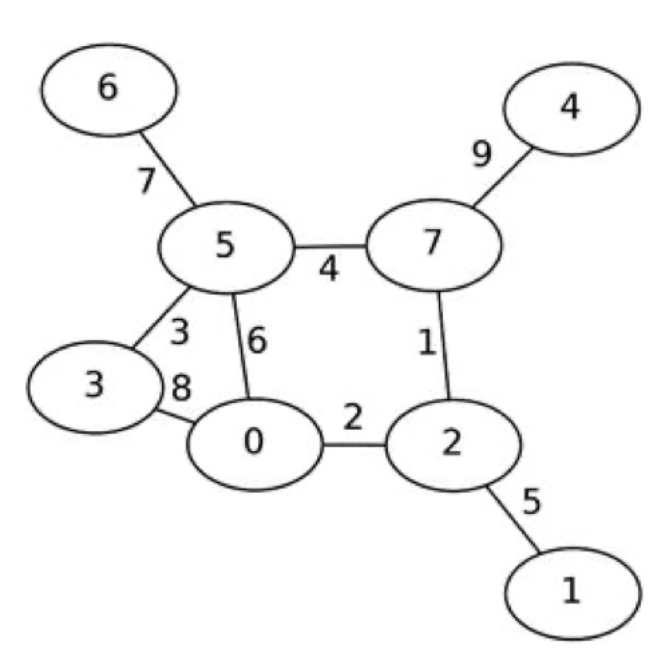
\includegraphics[width=.4\linewidth]{mst.png}
\end{figure}

\begin{solution}
%Write your answer here.
\begin{figure}[H]
    \centering
    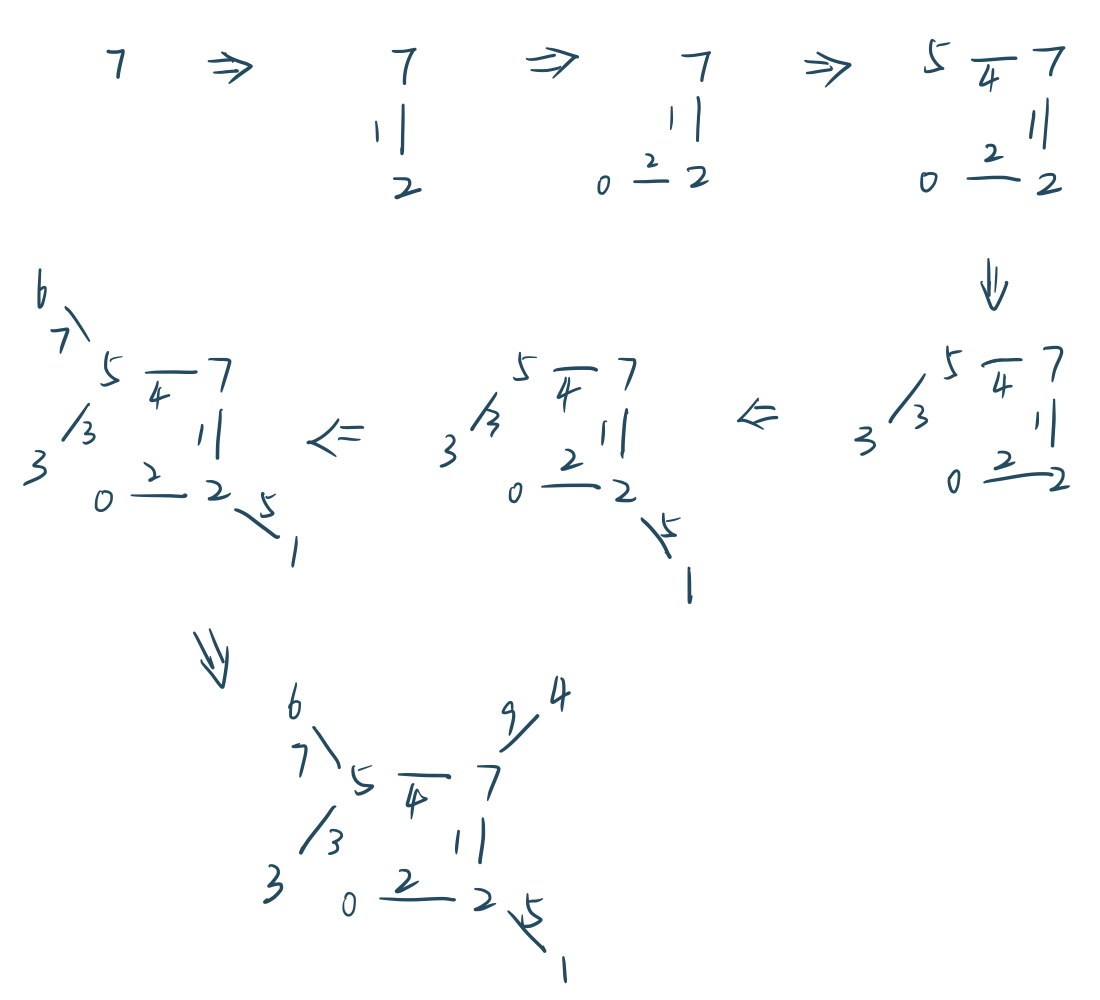
\includegraphics[width=.7\linewidth]{1.png}
\end{figure}
\end{solution}

\newpage
\section{Dynamic Programming (60 points)}
\textbf{\huge\color{red}All the problems in this part should be written in 15 lines in C++!}
\subsection{Minimum Nodes in an AVL Tree (20 points)}
You are given an AVL tree of height $h$. Write a function that returns the minimum number of nodes the AVL tree of height $h$ can have, For this problem, \textbf{assume that a tree with height 1 only has one node.}\\

\textbf{Hint: }Since AVL trees must be balanced, the height of each node's left and right children cannot have a difference that exceeds 1. 

\textbf{Example: }If $h$ is 3, then your function should return 4, since the smallest possible AVL tree with height 3 has 4 nodes.

\textbf{Complexity requirement:} $O(h)$ time and $O(h)$ auxiliary memory.

You can simply write your answer below. (No need to submit a code file)

\begin{solution}
\begin{lstlisting}[language=c++]
int min_nodes_in_AVL(int h) {
    vector<int>main_nodes_num(h+1,0);
    min_nodes_num.at(0) = 0;
    min_nodes_num.at(1) = 1;
    min_nodes_num.at(2) = 2;
    for(int i = 2; i < h+1; ++i){
        min_nodes_num.at(i) = min_nodes_num.at(i-1) + min_nodes_num.at(i-2) + 1;
    }
    return min_nodes_num.at(h-1);
}
\end{lstlisting}
\end{solution}

\subsection{Largest Distance Between Repeated Elements (20 points)}
You are given an array with repeated elements. Implement a function that identifies the maximum distance between any two occurrences of a repeated element.\\

\textbf{Example:} Given the following input:
\begin{align*}
\{1,2,3,2,2,1,3,3,2\}
\end{align*}

Your function should return 7, since the maximum distance between any two repeated elements is the distance between the 2 at index 1 and the 2 at index 8 or 8-1=7.

\textbf{Complexity requirement:} $O(n)$ time and $O(n)$ auxiliary memory, where $n$ is the length of the array.
\textbf{Hint:} Think carefully about what to store in the auxiliary memory!

\begin{solution}
\begin{lstlisting}[language=c++]
int max_repeated_distance(const vector<int> &vec) {
    unordered_map<int, int> dis;
    int max_dis = 0;
    for(int i = 0; i < vec.size(); ++i){
        if(dis.find(vec.at(i) == dis.end())){
            dis[vec.at(i)] = i;  // the first index when an element appear
        } else {
            max_dis = max(max_dis,i-dis[vec.at(i)]);
        }
    }
    return max_dis;
}
\end{lstlisting}
\end{solution}

\subsection{Tiling (20 points)}

Roihn is given a $2\times n$ board ($n>0$). He is interested in the number of \textbf{distinct} ways to tile the given board using tiles of dimensions ($2\times 1$), ($1\times 2$), ($2\times 1$), ($2\times 2$) as shown below:
\begin{figure}[H]
\centering
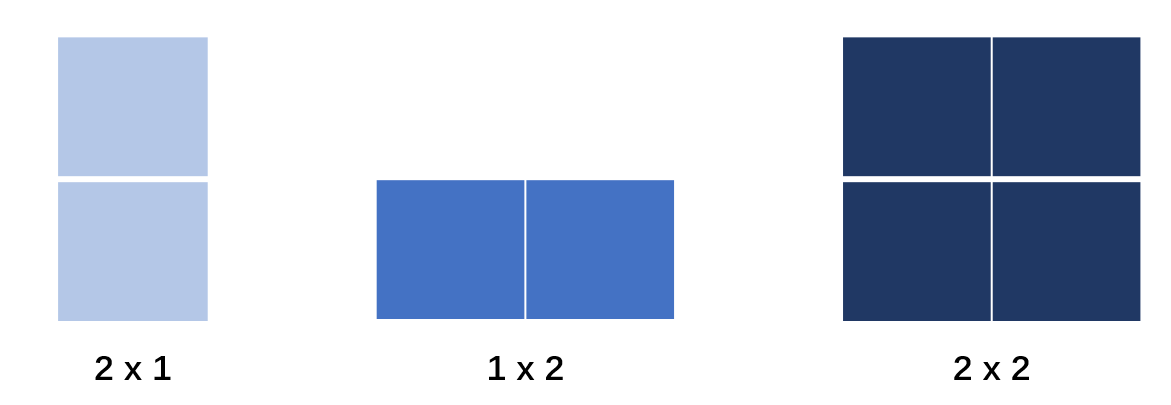
\includegraphics[width=.7\linewidth]{tile.png}
\end{figure}
For example, for a $2\times 2$ (i.e. $n=2$) board, there are 3 ways:
\begin{figure}[H]
\centering
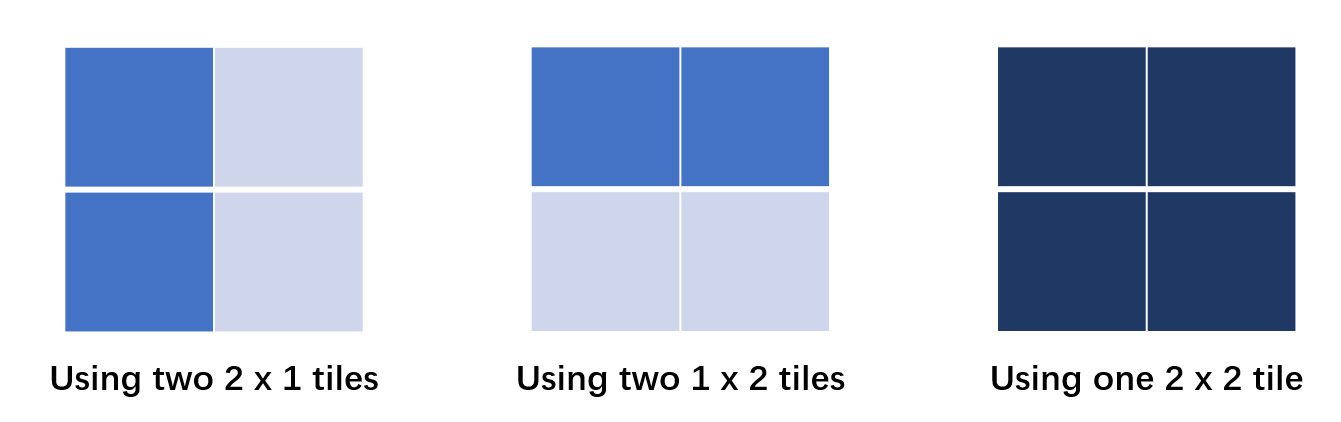
\includegraphics[width=.8\linewidth]{tile2x2.png}
\end{figure}

\textbf{Complexity requirement:} $O(n)$ time and $O(n)$ auxiliary memory

\begin{solution}
\begin{lstlisting}[language=c++]
int number_of_tilings(int n) {
    vector<int> ways_num = (n,0);
    ways_num.at(0) = 1;
    ways_num.at(1) = 3;
    for(int i = 2; i < n; ++i){
        ways_num.at(i) = ways_num.at(i-1)+2*ways_num.at(i-2);
    }
    return ways_num.at(n-1);
}
\end{lstlisting}
\end{solution}
\section*{Reference}
Assignment 4, VE281, FA2020, UMJI-SJTU.



\end{document}











